
%%--------------------------------------------------------------------------
%% Appendix
%%--------------------------------------------------------------------------

\begin{appendices}
\section{Appendix}\label{sec:appendix}
\subsection{More informative \& least as powerful test}\label{app:test-power}

See~\cref{fig:test-power}

\begin{figure}[!ht]
	\centering
	\begin{subfigure}[b]{\textwidth}
		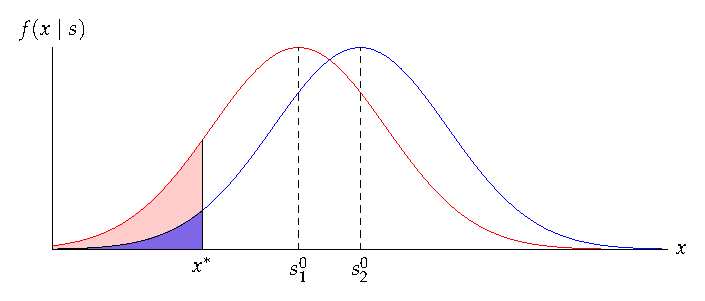
\includegraphics[width=\textwidth]{test-power-1.pdf}
		\caption{}\label{fig:test-power-1}
	\end{subfigure}
	\begin{subfigure}[b]{\textwidth}
		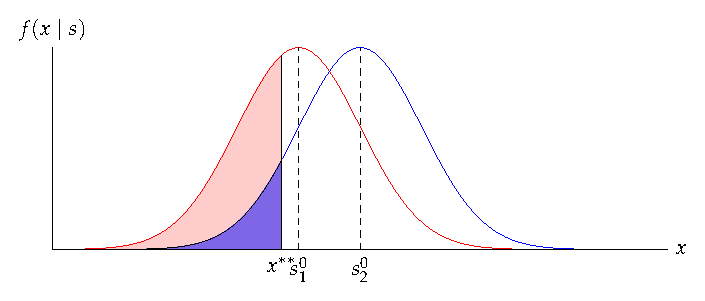
\includegraphics[width=\textwidth]{test-power-2.pdf}
		\caption{}\label{fig:test-power-2}
	\end{subfigure}
\caption{The blue shaded area is the probability of a type I error, and the red shaded area is the test power, while the non-shaded area under the red curve is the probability of a type II error. \Cref{fig:test-power-1,fig:test-power-2} have the same probability of a type I error, but the power of the test in \cref{fig:test-power-2} is higher than in \cref{fig:test-power-2}, as the probability of a type II error is smaller}\label{fig:test-power}
\end{figure}

%%--------------------------------------------------------------------------
%% Appendix: Stochastic Affiliation
%%--------------------------------------------------------------------------

\subsection{Stochastic Affiliation}\label{app:affiliation}
\begin{definition}
	The random variables $X_1,\ldots,X_n$ are said to be affiliated if their joint PDF $f(\mathbf{x})$ is log-supermodular, meaning that for  all $\mathbf{x},\mathbf{x}'\in\mathbb{R}_nb$, we have
	\[
		f(\mathbf{x}\land \mathbf{x}')f(\mathbf{x}\lor \mathbf{x}')\geq f(\mathbf{x})f(\mathbf{x}')
	\]
When $f$ is twice continuously differentiable, then equivalently $bX_1,\ldots,X_n$ are affiliated iff for all $i\ne j$
\[
	\frac{\partial^2}{\partial x_i \partial x_j}\ln f\geq 0
\]
\end{definition}
Consider two joint random variables $X$ and $S$. Affiliation then tells us about the conditional distribution of $f(S\mid x)$. If $x\leq x', y\leq y'$, then affiliation implies that
\[
	\frac{f(x,y')}{f(x,y)}\leq \frac{f(x',y')}{f(x',y)}
\]
which we can rewrite as
\[
	\frac{f(y'\mid x)f_X(x)}{f(y\mid x)f_X(x)}=\frac{f(y'\mid x)}{f(y\mid x)}\leq \frac{f(y'\mid x')}{f(y\mid x')} = \frac{f(y'\mid x')f_X(x')}{f(y\mid x')f_X(x')}
\]
which tells us the that likelihood ratio $f(\cdot\mid x)\big/ f(\cdot\mid x)$ is increasing in $x$ and thereby displays the monotone likelihood ratio property, which implies first-order (and hence second-order) stochastic dominance. \cite[in proposition 8 and 10 ]{Quah2009Comparative}, proofs that the monotone likelihood ratio property is required for the family of functions with the single-crossing property to have an increasing optimal solution in the signal $x$.

A further property of affiliation is that it is preserved under Bayesian updating, such that if the prior $f(s')\big/f(s),\, s'\geq s$ has a monotone likelihood ratio property, then the posterior $f(s'\mid x)\big/f(s\mid x)$ also have the monotone likelihood ratio property for any likelihood function $f(x\mid \cdot)$.

At last, affiliation is also preserved under multiplication, such that if $f(\mathbf{x})=h(\mathbf{x})g(\mathbf{x})$, where $g$ and $h$ is nonnegative and affiliated, then $f$ is also affiliated.
%%--------------------------------------------------------------------------
%% Appendix: Proof Topiks
%%--------------------------------------------------------------------------

\subsection[A simplified proof of Topkis’s Monotonicity Theorem is]{A simplified proof of \Citeauthor{Topkis1998Supermodularity}'s Monotonicity Theorem}\label{app:topiks-proof}
\begin{theorem}
	Consider the problem
	\[
		t^*(s)=\argmax_{s\in S} u(t,s)
	\]
	where $T,S\in \mathbb{R}$ and $T_s\subset T$ is the correspondence from $S$ to $T$  with $T_s$ being the set of feasible treatments, when the diseases is $s$.  Assume also that
	\begin{enumerate}[label=(\roman*)]
		\item $u$ has increasing differences in $(t,s)$  and
		\item $T_s=[g(s),h(s)]$  where $h,g:S \rightarrow \mathbb{R}$ are increasing functions with $g\leq h$
	\end{enumerate}
	Then the maximal and minimal selection of $t^*(s)$, $\bar{t}(s)$ and $\underbar{t}(s)$ is an increasing functions.
\end{theorem}

\begin{proof}
	The proof is done by contradiction. Assume that $\bar{t}(s)$ is not increasing. Then for some $s'>s$  $\bar{t}(s')<\bar{t}(s)$.  Then using assumption (ii) and the fact that $\bar{t}(s)\in T_s$  and $\bar{t}(s')\in T_{s'}$  it follows that $g(s)\leq g(s')\leq \bar{t}(s') < \bar{t}(s) \leq h(s) \leq h(s')$  so that $\bar{t}(s)\in T_{s'}$ and $\bar{t}(s')\in T_s$.  Using the latter facts along with $\bar{t}(s)\in t^*(s)$ and $\bar{t}(s')\in t^*(s')$  we have
	\begin{alignat*}{3}
	   & 0 && \geq u[s',\bar{t}(s)]-u[s',\bar{t}(s')] && \qquad \text{By optimality of } \bar{t}(s') \\
	   &   && \geq u[s,\bar{t}(s)]-u[s,\bar{t}(s')]   && \qquad \text{by increasing differences *} \\
	   &   && \geq 0                                  && \qquad \text{by optimality of } \bar{t}(s)
	\end{alignat*}
	which holds throughout. Hence it follows that $u(s',\bar{t}(s))=u(s',\bar{t}(s'))$, such that $\bar{t}(s)\in t^*(s')$, which is a contradiction to the fact that $\bar{t}(s')=\max \{t^*(s')\}$ in the view of $\bar{t}(s')<\bar{t}(s)$.  Hence, $\bar{t}(s)$ is an increasing function. The proff for $\underbar{t}(s)$ is symmetric \parencite{Amir2005Supermodularity}.\footnote{In this proof, it is assumed that $T_s\cap T_{s'}\ne \emptyset$. If this was the case, one would have that $\sup T_s < \inf T_{s'}$ and it follows trivially have that $t^*(s)<t^*(s')$}
\end{proof}
\subsection{The inverse of a strictly convex function is concave} % (fold)
\label{sub:the_inverse_of_a_strictly_convex_function_is_concave}
\begin{theorem}
Let $f$ be a real function which is convex on the open interval $I$, and let $J=f(I)$. Then if $f$ is strictly increasing on $I$, then $f^{-1}$ is concave on $J$.
\end{theorem}
 \begin{proof}
 Let $X=f(x)\in J$ and $Y=f(y)\in J$. From the definition of a convexity, it follows that $\forall a,b\in \mathbb{R}_{++}, a+b=1:f(ax+by)\leq af(x)+bf(y)$. 

Let $f$ be increasing on $I$. Then $f^{-1}$ is increasing on $J$, as the inverse of a monotone increasing function is increasing. Thus, $af^{-1}(X)+bf^{-1}(Y)=ax+by\leq f^{-1}(aX+bY)$, and hence $f^{-1}$ is concave on $J$
 \end{proof}
% subsection the_inverse_of_a_strictly_convex_function_is_concave (end)


\end{appendices}
